%Type document
\documentclass[a4paper, 12pt, titlepage]{report}

%Taal: Nederlands ("Inhoudsopgave", "Hoofdstuk",...)
\usepackage[dutch]{babel}

%Geen nummering bij secties en hoofdstukkden
\setcounter{secnumdepth}{-1} 

%De diepte van de inhoudsopgave
\setcounter{tocdepth}{2}

%Marges
\usepackage[left=2cm,top=2cm,right=2cm,bottom=2cm,a4paper]{geometry}

%Bijschriften kleiner lettertype geven (dit moet voor \usepackage{subfig} staan)
\usepackage[footnotesize]{caption}

%Figuren
\usepackage{graphicx}

%Meerdere figuren naast elkaar (met apart bijschrift)
\usepackage{subfig}
\usepackage{subfloat}

%Lettertype sans-serif, charter
%\renewcommand{\familydefault}{\sfdefault}
%\usepackage{charter}

%Lettertype hoofdstuktitels
%\usepackage{sectsty}
%\chapterfont{\fontfamily{cmr}\fontseries{b}\fontsize{25pt}{30pt}\selectfont}
%\sectionfont{\fontfamily{cmr}\fontseries{b}\fontsize{20pt}{25pt}\selectfont}
%\subsectionfont{\fontfamily{cmr}\fontseries{b}\fontsize{15pt}{20pt}\selectfont}
%\subsubsectionfont{\fontfamily{cmr}\fontseries{b}\fontsize{11pt}{20pt}\selectfont}

%Nummering voetnoten niet resetten bij nieuw hoofdstuk
\usepackage{remreset}
\makeatletter\@removefromreset{footnote}{section}\makeatother

%Hyperlinks
\usepackage{hyperref}

%Opmaak hyperlinks
\hypersetup{colorlinks=false,	urlcolor=cyan,pdfborder=0 0 0}

%Koptekst, voettekst, paginanummers
\usepackage{fancyhdr}
	
%Type paginastijl
\pagestyle{fancy}

%Paginanummers
\fancypagestyle{plain}

%Paginanummers rechtsonder
\fancyfoot[R]{\thepage}

%Geen paginanummers centraal onder
\fancyfoot[C]{}

%Geen koptekst
\fancyhead{} 

%Geen randen aan koptekst/voettekst
\renewcommand{\headrulewidth}{0pt}
\renewcommand{\footrulewidth}{0pt}

%Voettekst naar boven
\setlength\voffset{-0.25in}

%Teksthoogte
%\setlength\textheight{700pt}

%Hoogte van de voettekst
\setlength\footskip{50pt}

%"Figuur" in vet
\makeatletter
\renewcommand{\fnum@figure}{\small\textbf{\figurename~\thefigure}}
\makeatother

\usepackage{titling}
\newcommand{\subtitle}[1]{%
  \posttitle{%
    \par\end{center}
    \begin{center}\large#1\end{center}
    \vskip0.5em}%
}

%Titelblad
\author{Martijn Bouss\'e\\
	{Dario Incalza}\\
	{\em Faculteit Ingenieurswetenschappen}\\
	{\em Katholieke Universiteit Leuven}
}

\title{Numerieke Modellering en Benadering\\
	{Practicum 1: Eigenwaardenproblemen}
}

\date{woensdag 24 april 2013}

%Witruimte tussen alineas, niet inspringen
\setlength{\parindent}{0pt}
\setlength{\parskip}{1.5ex plus 0.5ex minus 0.2ex}

%weergave euroteken
\usepackage{eurosans}
\usepackage[official]{eurosym}

%wiskunde typen
\usepackage{amsmath, amssymb, textcomp, mathtools}

%om tabellen te kleuren
\usepackage[table]{xcolor}

\usepackage[final]{pdfpages}

%pseudo-code
\usepackage{algorithmic}

%graden symbool
\newcommand{\degree}{\ensuremath{^\circ}}

\usepackage{listings}
\lstset{
language=Matlab, % choose the language of the code
%basicstyle=10pt, % the size of the fonts that are used for the code
numbers=left, % where to put the line-numbers
numberstyle=\footnotesize, % the size of the fonts that are used for the line-numbers
stepnumber=1, % the step between two line-numbers. If it's 1 each line will be numbered
numbersep=5pt, % how far the line-numbers are from the code
%backgroundcolor=\color{grey}, % choose the background color. You must add \usepackage{color}
showspaces=false, % show spaces adding particular underscores
showstringspaces=false, % underline spaces within strings
showtabs=false, % show tabs within strings adding particular underscores
frame=single, % adds a frame around the code
%tabsize=2, % sets default tabsize to 2 spaces
%captionpos=b, % sets the caption-position to bottom
breaklines=true, % sets automatic line breaking
breakatwhitespace=false, % sets if automatic breaks should only happen at whitespace
escapeinside={\%*}{*)} % if you want to add a comment within your code
}






%%%%%%%%%%%%%%%%%%%%%%%%%%%%%%%%%%%%%%%%%%%%%%%%%%%%
\begin{document}

\maketitle

\tableofcontents

\listoffigures

\pagebreak

\section{Inleiding}
In het kader van het vak Numerieke Modellering en Benadering worden in dit practicum methoden voor het bepalen van eigenwaarden van volle matrices onderzocht. In een eerste gedeelte worden enkele theoretische eigenschappen van de methoden beschouwd. Vervolgens worden de convergentie-eigenschappen van deze methoden in het tweede deel nader onderzocht aan de hand van enkele MATLAB-experimenten. Ten slotte wordt in een derde gedeelte \'e\'en van de alternatieve eigenwaardenalgoritmen, met name de bisectie-methode, in meer detail bekeken.

\section{Theoretische eigenschappen}

\subsection{Opgave 1}
\paragraph{a)} Om alle eigenwaarden van een symmetrische matrix $A \in \mathbb{R}^{m\times m}$ te vinden gebruiken we het QR-algoritme. Om het algoritme praktisch bruikbaar te maken dienen er enkele aanpassingen te gebeuren aan het basis algoritme. E\'en van de belangrijkste aanpassing is het gebruiken van shifts. Het volledig algoritme wordt gegeven als:\\

\begin{algorithmic}[frame=single]
 \STATE $(Q^{(0)})^TA^{(0)}Q^{(0)}$
 \FOR {$k=1,2,...$} 
 	\STATE Kies een shift $\mu^{(k)}$
 	\STATE $Q^{(k)}R^{(k)} = A^{(k-1)}-\mu^{(k)}I$
 	\STATE $A^{(k)} = R^{(k)}Q^{(k)}+\mu^{(k)}I$
 	\IF {Een niet-diagonaal element $A^{(k)}_{j,j+1}$ dicht genoeg bij nul is} 
 		\STATE kies $A_{j,j+1} = A_{j+1,j} = 0 $ en zo bekom je,
 		\STATE $\begin{bmatrix} A_1 & 0 \\ 0 & A_2 \end{bmatrix} = A^{(k)}$
 		\STATE Pas het QR-algoritme toe op $A_1$ en $A_2$
 	\ENDIF
 \ENDFOR
\end{algorithmic}

Alvorens dit algoritme toegepast wordt, dient er opgemerkt te worden dat $A$ gereduceerd wordt tot een tridiagonale vorm. Door deze reductie toe te passen worden er nullen toegevoegd zowel in de rijen als in de kolommen, op deze manier worden overbodige arithmetische operaties vermeden. Dit bevordert aanzienlijk de rekenkost dat nodig is om het algoritme uit te voeren.

Men kan het Rayleigh quoti\"ent toe passen op de laatste kolom van $Q^{(k)}$, we krijgen dan:

\begin{equation}
	\mu^{(k)} = \frac{(q^{(k)}_m)^TAq^{(k)}_m}{(q^{(k)}_m)^Tq^{(k)}_m} = (q^{(k)}_m)^TAq^{(k)}_m
	\label{eqn:rayleighquotient}
\end{equation}

Door dit getal, $\mu^{(k)}$, te kiezen als shift in elke stap zal $q^{(k)}_m$ kubisch gaan convergeren naar een eigenvector. Naast de \emph{Rayleigh shift} kan men ook de \emph{Wilkinson shift} toepassen. Het is \'e\'envoudig aan te tonen dat \emph{kubische convergentie} enkel in de, min of meer, algemene gevallen bereikt wordt. Er kan aangetoond worden dat de Wilkinson shift, minstens, \emph{kubische convergentie} bereikt in het slechtste geval. Beschouw matrix B waarbij Rayleigh shift niet zal werken en Wilkinson Shift wel,

\begin{equation}
 B = \begin{bmatrix} 0 & 1 \\ 1 & 0 \end{bmatrix}
\end{equation}

Het algoritme zal falen voor B, omdat de eigenwaarden van B symmetrisch rond de oorsprong liggen, $-1$ en $1$. De gebruikte schatter kan dan geen richting kiezen om naar toe te convergeren. Men gebruikt dan de Wilkinson Shift om de symmetrie te breken, waardoor een convergentie naar, in dit geval, -1 gevonden wordt. Het aantal flops nodig door het QR-algoritme met shifts bedraagt, bij benadering, $\frac{4}{3}m^3$ flops.

\paragraph{b)} Om de eigenwaarden te bepalen die het dichts gelegen zijn bij een bepaald getal $\beta$, van een symmetrische matrix $A\in \mathbb{R}^{m\times m}$, beschouwen we de \emph{Rayleigh quoti\"ent iteratie}. De Rayleigh quoti\"ent van een vector $x \in \mathbb{R}^m$ is de scalar:

\begin{equation}
	r(x) = \frac{x^TAx}{x^Tx}
\end{equation}

We kunnen dit geometrisch interpreteren als, de eigenvectors van A zijn de stationaire punten van de functie $r(x)$ en eveneens zijn de eigenwaarden van A de waarden van $r(x)$ ge\"evalueerd in deze stationaire punten.

Nu we het Rayleigh quoti\"ent gedefinie\"erd hebben, kunnen we overgaan tot het \emph{Rayleigh quoti\"ent iteratie algoritme}. Deze wordt gegeven als volgt:\\

\begin{algorithmic}
 \STATE $v^{(0)} = $een bepaalde vector waarvan de lengte gelijk is aan 1
 \STATE $\lambda^{(0)} = (v^{(0)})^TAv^{(0)}$, dit is het overeenkomende Rayleigh quoti\"ent
 \FOR{$k=1,2,...$} 
 	\STATE Los $(A-\lambda^{(k-1)}I)w = v^{(k-1)}$ op naar $w$
 	\STATE $v^{(k)} = \frac{w}{\mid \mid w \mid \mid}$
 	\STATE $\lambda^{(k)}=(v^{(k)})^TAv^{(k)}$
 \ENDFOR
\end{algorithmic}

Dit algoritme kan intu\"itief beschouwd worden door te beredeneren dat we constant de schattingen van de eigenwaarden beter gaan proberen uit te voeren. Hierdoor zal de convergentie van de inverse iteratie stijgen in elke stap. Elke iteratie verdrievoudigd de nauwkeurigheid. Meer nog, er kan bewezen worden dat de convergentie kubisch is. Voor het bewijs verwijzen we naar theorema 27.3 op pagina 208 in het boek Numerical Linear Algebra. Het aantal flops nodig voor Rayleigh Quotient Iteratie bedraagt $O(m^3)$, indien we de matrix eerst in zijn tridiagonale vorm zetten spreken we nog over $O(m)$ flops.


\subsection{Opgave 2}
\paragraph{a)} Gegeven een matrix $A \in \mathbb{R}^{m \times m}$ en een vector $x \in \mathbb{R}^{m \times 1}$, waarbij $x$ een benadering is voor een eigenvector van $A$. Welke scalar $\rho$ gedraagt zich het \emph{meeste} als een eigenwaarde voor $x$? Dit kan geformuleerd worden als een $m \times 1$ kleinste kwadraten probleem van de vorm $x \rho \approx Ax$, waarbij $Ax$ het rechterlid voorstelt, $x$ de matrix en $\rho$ de onbekende vector. Beschouw de volgende doelfunctie:
\begin{equation}
	f(\rho) = \frac{1}{2}|| Ax-x\rho ||^{2}_{2}
\end{equation}
en volgend optimalisatieprobleem zonder beperkingen:
\begin{equation}
\begin{aligned}
& \underset{\rho \in \mathbb{R}}{\text{min}}
& & f(\rho) \\
\end{aligned}
\end{equation}
Aangezien $f(\rho)$ convex is, wordt het minimum gevonden als een stationair punt van de doelfunctie:
\begin{equation}
	\nabla f(\rho) = 0 \Leftrightarrow \frac{1}{2}\nabla \begin{pmatrix} x^{T}A^{T}Ax - 2\rho x^{T}Ax + \rho^{2}x^{T}x \end{pmatrix} = 0 \Leftrightarrow \frac{1}{2} \begin{pmatrix} -2x^{T}Ax + 2\rho x^{T}x \end{pmatrix} = 0
\end{equation}
Dit levert exact de definitie van de Rayleigh quoti\"ent van $x$:
\begin{equation}
	r(x) = \rho = \frac{x^{T}Ax}{x^{T}x}
\end{equation}

\paragraph{b)} De Rayleigh quoti\"ent methode lost in elke iteratie het stelsel $(A-\lambda^{(k-1)}I)w = v^{(k-1)}$ op. Dit stelsel wordt steeds meer en meer singulier naarmate de benaderende eigenwaarde $\lambda^{(k-1)}$ dichter in de buurt van de exacte eigenwaarde komt. Merk echter op dat de term $-\lambda^{(k-1)}I$ de gezochte eigenwaarde zeer klein maakt, waardoor bij het oplossen van het stelsel de richting zeer sterk zal benadrukt worden. De vector $w$ zal daardoor ook zeer groot worden, maar nog steeds in de juiste richting wijzen. 


\subsection{Opgave 3}
Gelijktijdige iteratie past de methode van de machten toe op meerdere kolommen tegelijk. Op die manier kunnen de $n$ grootste eigenwaarden van een matrix $A$ bepaald worden. Indien $A$ niet singulier is kunnen de $n$ kleinste eigenwaarden gevonden worden door de methode van de machten met de inverse van de matrix $A$ toe te passen. Beschouw de volgende pseudo-code:\\

\begin{algorithmic}
\STATE Initialiseer $\hat{Q}^{(0)} \in \mathbb{R}^{m \times n}$ met $n$ orthonormale kolommen.
\FOR	 {$k = 1,2,...$}
\STATE $Z = A^{-1}\hat{Q}^{k-1}$
\STATE $\hat{Q}^{k}\hat{R}^{k} = Z$
\ENDFOR
\end{algorithmic}

Om in te zien dat dit algoritme werkt kunnen we analoog aan pagina 213 in Numerical Linear Algebra werken. Neem dezelfde veronderstellingen en symbolen aan, dan kan nu $v_{j}^{k}$ geschreven worden als:

\begin{equation}
	v_{j}^{k} = a_{1j}\lambda_{1}^{-k}q_{1} + ... + a_{mj}\lambda_{m}^{-k}q_{m}
	\label{eq:vjk}
\end{equation}

Vergelijking~\ref{eq:vjk} toont aan dat nu de kleinste eigenwaarden de grootste waarden worden en dat bijgevolg de $n$ kleinste eigenwaarden uit het algoritme volgen. De daaropvolgende afleidingen zijn volledig analoog. Figuur~\ref{fig:opgave3} toont een eenvoudig MATLAB-experiment, waarbij de vier kleinste eigenwaarden van een matrix $A$ met spectrum $\Lambda = \{ 1, 2, ..., 10\}$ worden bepaald.

\begin{figure}[htb]
	\centering
	\includegraphics[width=0.6\textwidth]{figuren/opgave3.png}
	\caption{Convergentiegedrag van inverse gelijktijdige iteratie voor een eenvoudige matrix $A$ met spectrum $\Lambda = \{ 1, 2, ..., 10\}$. De vier kleinste eigenwaarden $\lambda = \{ 1, 2, 3, 4\}$ worden bepaald. De nauwkeurigheid op de kleinste eigenwaarde bereikt het eerst de machineprecisie.}
	\label{fig:opgave3}
\end{figure}



\section{Convergentie-experimenten}
In dit deel wordt een volle, re\"ele, symmetrische matrix $A$ beschouwd. In MATLAB wordt daarvoor de matrix \emph{mat1.txt} ingeladen met het commando \emph{load}.

\subsection{Opgave 4}
De gegeven matrix $A$ wordt gereduceerd naar Hessenberg vorm met behulp van het commando \emph{Hess}. Aan de hand van het commando \emph{spy} wordt in Figuur~\ref{fig:opgave4} de structuur van de bekomen matrix getoond. Merk echter op dat de resulterende matrix tridiagonaal is aangezien de originele matrix symmetrisch was. Inspecteer hiervoor de elementen van de matrix in MATLAB.

Methoden voor het bepalen van eigenwaarden zullen doorgaans werken in twee fasen. In een eerste fase gebruikt men een directe methode om de volle, symmetrische matrix $A \in \mathbb{R}^{m \times m}$ te structuren tot een tridiagonale matrix $H$. Deze directe reductie kost $\mathcal{O}(m^3)$ flops. In een tweede fase genereert men een oneindige sequentie van tridiagonale matrices die convergeren naar een diagonaalmatrix. Convergentie wordt meestal reeds bereikt in $\mathcal{O}(m)$ iteraties en per iteratie kost dit slechts $\mathcal{O}(m)$ flops. Bijgevolg kost deze tweede fase $\mathcal{O}(m^2)$ flops. Dit verklaart het belang van de eerste fase! Zonder de directe reductie wordt in de tweede fase telkens op een volle matrix ingewerkt, wat een verhoging van het aantal flops per iteratie inhoudt en bijgevolg het totaal aantal flops.

\begin{figure}[htb]
	\centering
	\includegraphics[width=0.4\textwidth]{figuren/opgave4.png}
	\caption{Structuur van de re\"ele, symmetrische matrix A na reductie. Inspecteer de elementen van de matrix om in te zien dat de structuur wel degelijk tridiagonaal is.}
	\label{fig:opgave4}
\end{figure}

\subsection{Opgave 5}
Wanneer we de drie methoden toe passen op de gegeven matrix, bekomen we Figuur~\ref{fig:opgave5}. We zien hier duidelijk dat het QR-algoritme zonder shifts een lineaire convergentie heeft en de QR-algoritmen die Rayleigh of Wilkinson shifts gebruiken een kubische convergentie hebben. Alvorens de convergentie te onderzoeken lichten we even toe waarom we residus gebruiken. We defini\"eren het residu als het element dat vlak boven een diagonaal element staat. Deze zal geleidelijk aan naar nul convergeren. We beschouwen de convergentie van deze residus om de convergentie van de verschillende algoritmen te bepalen. We zullen de huidige residus in elke stap evalueren ten opzichte van de vorige residus. 

Het QR-algoritme zonder shifts is conform met de theorie. Indien we theorema 28.4 beschouwen op pagina 218 in het boek Numerical Linear Algebra, komen we tot de vastelling dat dit algoritme een lineare convergentie heeft. Dit op voorwaarde dat de matrix waarop het algoritme toegepast wordt een re\"ele symmetrische matrix is.

Stel dat we het getal, dat besproken is in Vergelijking~\ref{eqn:rayleighquotient}, gebruiken als shift in elke iteratie stap dan bekomen we het QR-algoritme met Rayleigh shifts. In dat geval geld er dat de eigenwaarde en eigenvector schattingen, $\mu^{(k)}$ en $q^{(k)}_m$, identiek zijn aan deze die berekend worden door de Rayleigh quoti\"ent iteratie dat gestart wordt met $e_m$. Hieruit leiden we af dat het QR-algoritme dan een kubische convergentie heeft, omdat $q^{(k)}_m$ kubisch convergeert naar een eigenvector. Dit komt overeen met het resultaat op de figuur.

Het QR-algoritme met Rayleigh shifts is zeer gevoelig aan zijn begincondities. Niet in alle gevallen hebben we convergentie, daarom wordt Wilkinson shift gebruikt bij het QR-algoritme. We defini\"eren de Wilkinson shift als een eigenwaarde van een matrix $B$ dat het dichtst gelegen is bij $a_m$. Waarbij voor $B$ geldt:

\begin{equation}
B = \begin{bmatrix} a_{m-1} & b_{m-1} \\ b_{m-1} & a_m \end{bmatrix}
\end{equation}

Gelijkaardig aan de Rayleigh quoti\"ent shift bereikt ook de Wilkinson shift kubische convergentie. Meer nog, zelfs in het slechtste geval bereikt het gegarandeerd kubische convergentie. Dit wordt ook bevestigd op Figuur~\ref{fig:opgave5}.

\begin{figure}[htb]
	\centering
	\includegraphics[width=0.8\textwidth]{figuren/opgave5.png}
	\caption{Convergentiegedrag van het QR-algoritme zonder shift, met Rayleigh shift en met Wilkinson shift.}
	\label{fig:opgave5}
\end{figure}


\subsection{Opgave 6}
Figuur~\ref{fig:opgave6_1} illustreert het convergentiegedrag van het QR-algoritme met Rayleigh shift en Rayleigh quoti\"ent iteratie. Toepassing van theorema 27.3, op pagina 208 in Numerical Linear Algebra, leert ons dat Rayleigh quoti\"ent iteratie een kubische convergentie kent. Verder is er ook een verband aan te tonen tussen Rayleigh quoti\"ent shift en Rayleigh quoti\"ent iteratie.

\begin{figure}[htb]
	\centering
	\includegraphics[width=0.8\textwidth]{figuren/opgave6_1.png}
	\caption{Vergelijking van het convergentiegedrag van het QR-algoritme met Rayleigh shift ten opzichte van Rayleigh quoti\"ent iteratie.}
	\label{fig:opgave6_1}
\end{figure}

Wanneer we het QR algoritme met shifts beschouwen, hebben we een manier nodig om snelle convergentie te hebben in de laatste kolom $\underline{Q}^{(k)}$. We kunnen hiervoor het Rayleigh quoti\"ent gebruiken.

Indien we nu het bovenbeschreven verband beschouwen samen met bovenvernoemde theorema 27.3, komen we tot de vastelling dat beide algoritmen een kubische convergentie moeten vertonen, wat bevestigd wordt door Figuur ~\ref{fig:opgave6_1}.

\begin{figure}[htb]
	\centering
	\includegraphics[width=0.8\textwidth]{figuren/opgave6_2.png}
	\caption{Vergelijking van het convergentiegedrag van het QR-algoritme zonder shift ten opzichte van gelijktijdige iteratie.}
	\label{fig:opgave6_2}
\end{figure}

Het convergentiegedrag van het QR-algoritme zonder shift en gelijktijdige iteratie wordt getoond in Figuur~\ref{fig:opgave6_2}. Beschouwen we verder theorema 28.3, pagina 216 in het boek Numerical Linear Algebra, dan zien we een verband tussen het QR-algoritme zonder shift en het algoritme dat gelijktijdige iteratie gebruikt. Indien men het algoritme voor gelijktijdige iteratie beschouwt:\\ 

\begin{algorithmic}
 \STATE Kies $\hat{Q}^{(0)}\in \mathbb{R}^{m\times n}$ met orthonormale kolommen
 \FOR{$k=1,2,...$} 
 	\STATE $Z = A\hat{Q}^{(k-1)}$
 	\STATE $\hat{Q}^{(k)}\hat{R}^{(k)} = Z$
 \ENDFOR
\end{algorithmic}

Dan kan het verband aangetoond worden volgens voorgenoemde theorema als volgt. Beide algoritmen genereren dezelfde matrices $\underline{R}^{(k)},\underline{Q}^{(k)} en \underline{A}^{(k)}$. Meer nog, dit zijn de matrices gevonden door het uitvoeren van een QR-factorisatie van de k-de macht op de matrix A.

Volgens theorema 28.4, pagina 218 in het boek Numerical Linear Algebra, is de convergentie van een QR-algoritme zonder shifts lineair. Samen met het bovengenoemde verband en theorema 28.4 stellen we vast dat beide algoritmen lineair convergeren. Figuur ~\ref{fig:opgave6_2} bevestigt de redenering.


\subsection{Opgave 7}
We genereren een ijle $1000\times 1000$ matrix. Wanneer we Arnoldi toepassen op deze matrix en vervolgens de Ritz waarden berekenen in elke stap dan verkrijgen we Figuur ~\ref{fig:arnoldi}.

\begin{figure}[htb]
	\centering
	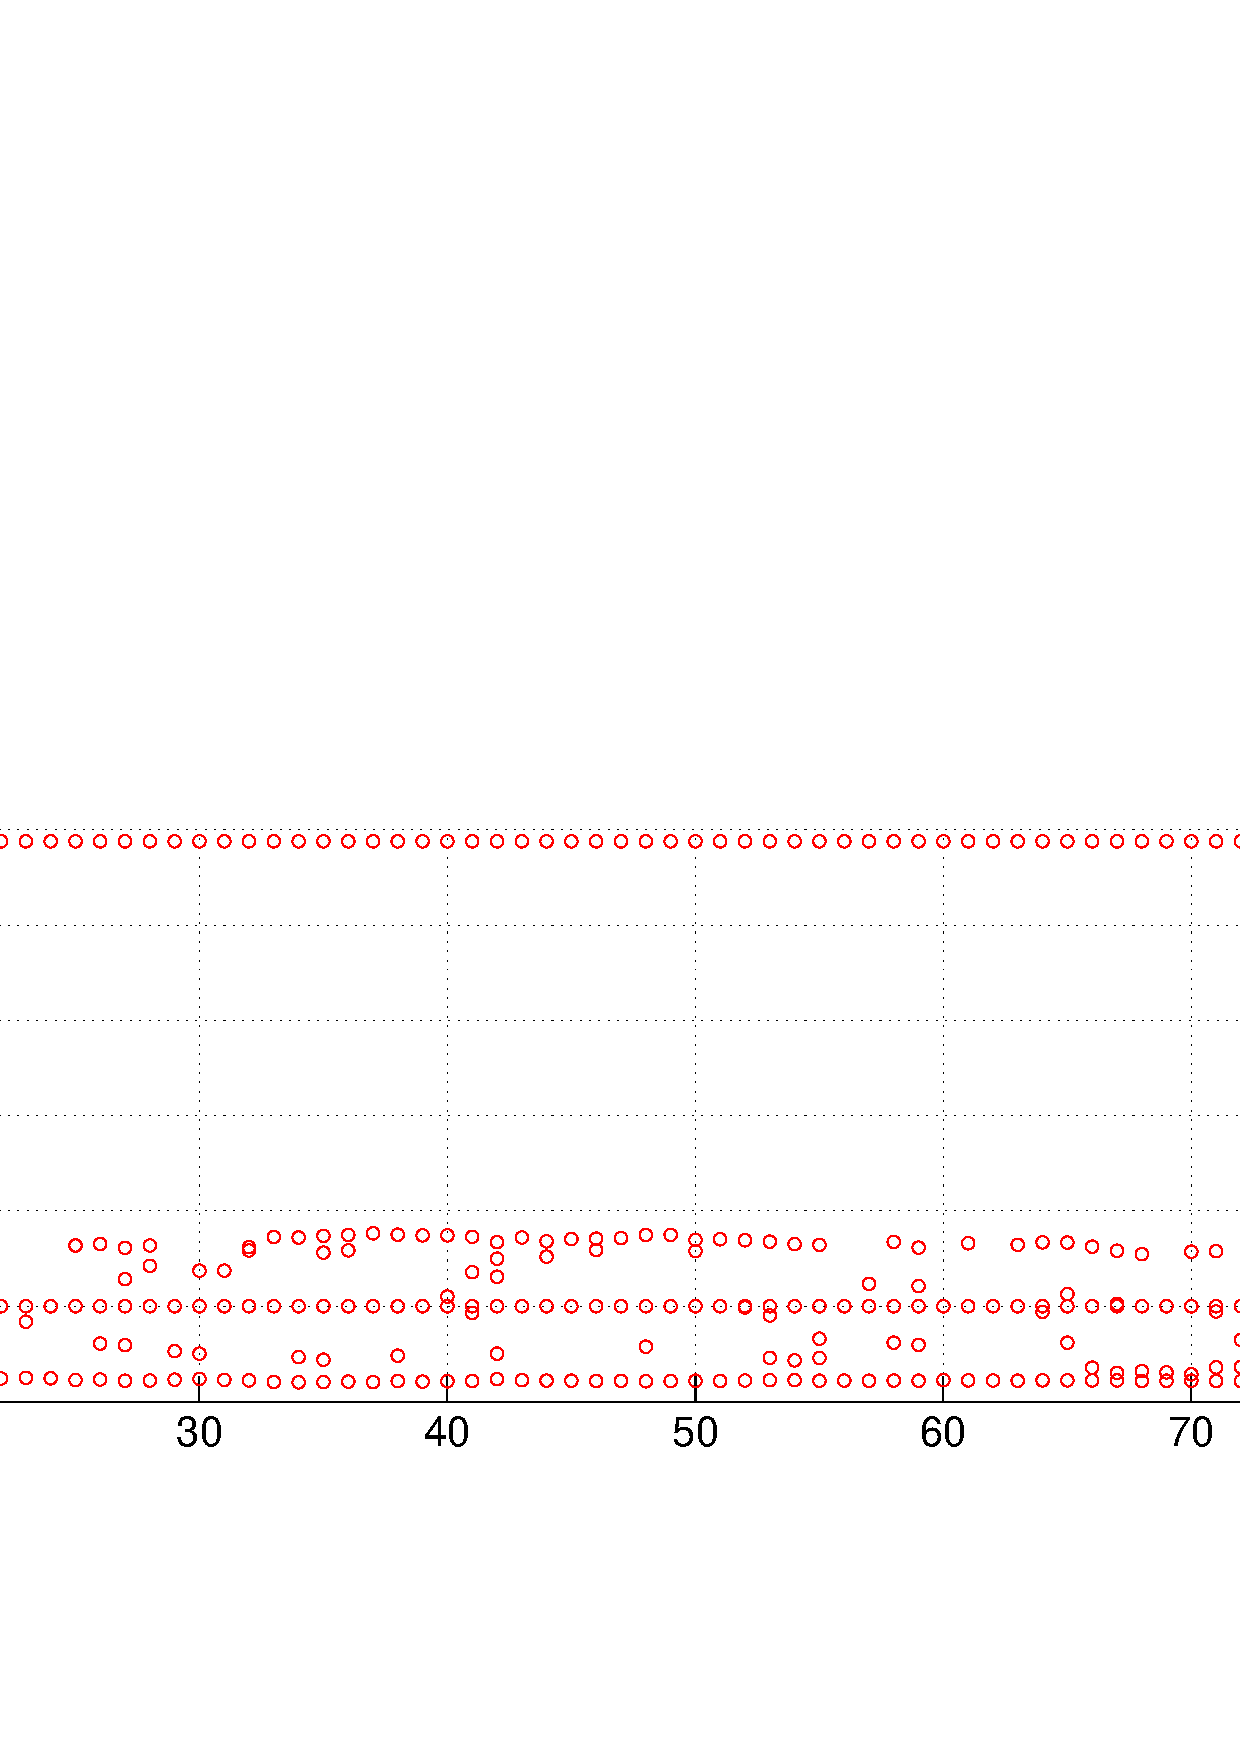
\includegraphics[width=0.8\textwidth]{figuren/arnoldi.png}
	\caption{Illustratie van de convergentie van de Arnoldi-Ritz waarden.}
	\label{fig:arnoldi}
\end{figure}

Wanneer we de eigenwaarden van de matrix berekenen met het commando $eigs(A)$ verkrijgen we als extreme eigenwaarde $24.3530$, de figuur convergeert inderdaad naar deze eigenwaarde toe. Er dient opgemerkt dat Arnoldi niet altijd convergeert naar alle eigenwaarden, enkel naar de extremen. Wanneer we Figuur  ~\ref{fig:arnoldi} beschouwen zien we dat de Arnoldi iteratie veel sneller convergeert voor de extreme eigenwaarde dan voor de eigenwaarden die aanzienlijk kleiner zijn dan de extreme eigenwaarde. We zien hier duidelijk een geometrische convergentie naar de extreme eigenwaarde. 


\section{Alternatieve eigenwaardenalgoritmen}

\subsection{Opgave 8}
Beschouw een symmetrische matrix $A \in \mathbb{R}^{m \times m}$ met $A^{(1)}, A^{(2)}, ..., A^{(m)}$ de linksboven vierkante submatrices van dimensies $1, 2,...,m$. Neem verder aan dat $A$ tridiagonaal is en dat de elementen van de nevendiagonalen verschillend zijn van nul:

\begin{equation}
	A = \begin{pmatrix} a_1 & b_1 & 0 			& 0 			&					\\ 
											b_1 & a_2 & b_2 		& 0 			&					\\ 
											  	& b_2 & a_3 		& \ddots 	&					\\
												 	&   	& \ddots 	& \ddots 	&	b_{m-1}	\\
												 	&			&					&	b_{m-1}	&	a_m			\end{pmatrix}
\end{equation}

De eigenwaarden van de submatrix $A^{(k)}$ zijn allen verschillend en worden genoteerd als: $\lambda^{(k)}_{1} < \lambda^{(k)}_{2} < ... < \lambda^{(k)}_{k}$. De eigenwaarden van de verschillende submatrices \emph{interlacen} strikt als volgt:

\begin{equation}
	\lambda^{(k+1)}_{j} < \lambda^{k}_{j} < \lambda^{(k+1)}_{j+1}
\end{equation}

Voor $k = 1,2,...,m-1$ en $j = 1,2,...,k-1$. Het is net deze eigenschap die het mogelijk maakt om het aantal eigenwaarden van een matrix in een interval te bepalen.

Beschouw bij wijze van voorbeeld de symmetrische matrix $A \in \mathbb{R}^{4 \times 4}$:

\begin{equation}
	A = PLP^{T}
\end{equation}

met $P$ een willekeurige orthogonale matrix, geconstrueerd met de commando's \emph{orth} en \emph{rand}, en $L$ gedefinieerd als volgt:

\begin{equation}
	L = \begin{pmatrix} 1 & 0 & 0 & 0 \\ 
											0 & 2 & 0 & 0 \\ 
											0 & 0 & 3 & 0 \\
											0 & 0 & 0 & 4 \end{pmatrix}
\end{equation}

Figuur~\ref{fig:opgave8} illustreert de \emph{interlacing} voor de eigenwaarden van de overeenkomstige submatrices. 

\begin{figure}[htb]
	\centering
	\includegraphics[width=0.5\textwidth]{figuren/opgave8.png}
	\caption{Illustratie van de \emph{interlacing}-eigenschap voor een eenvoudige re\"ele, symmetrische matrix $A$ met spectrum $\Lambda = \{1,2,3,4\}$.}
	\label{fig:opgave8}
\end{figure}

\subsection{Opgave 9}
Dit gedeelte beschrijft in pseudo-code het algoritme van de bisectie-methode om alle eigenwaarden van een symmetrische matrix $A \in \mathbb{R}^{m \times m}$ in een interval $[a,b)$ te bepalen. Voor alle duidelijkheid wordt het algoritme beschreven door twee kleinere algoritmes. Een eerste pseudo-code beschrijft een manier om de tekenwissels te tellen in de Sturm-sequentie, een tweede beschrijft de klassieke bisectie-methode met behulp van het vorige.

Uit de \emph{interlacing}-eigenschap, beschreven in de vorige opgave, volgt de Sturm sequentie (veronderstel dezelfde aannames als in de vorige opgave):

\begin{equation}
	p^{(k)}(x) = (a_k - x)p^{(k-1)}(x)-b_{k-1}^{2}p^{(k-2)}(x)
	\label{eq:sturm}
\end{equation}

Definieer $p^{(0)}=1$ en $p^{(1)}=a_k-x$ opdat dit geldig is voor $k = 2,3,...,m$. Indien Vergelijking~\ref{eq:sturm} meermaals wordt toegepast op verschillende waarden voor $x$ en daarbij de tekenwissels in de sequentie worden geteld, kan hierbij het aantal eigenwaarden binnen een interval bepaald worden. Beschouw nu de volgende pseudo-code:\\

\begin{algorithmic}
\STATE Initialiseer de Sturm sequentie.
\STATE $p^{(0)}=1, p^{(1)}=a_k-x$
\STATE Initialiseer de teller.
\STATE $t = 0$
\IF 	 {$p^{(0)}p^{(1)}<0$}
\STATE $t = 1$
\ENDIF	
\FOR 	 {$k = 2,3,...,n$}
\STATE Bereken het volgende element uit de Sturm sequentie.
\STATE $p^{(k)} = (a_k - x)p^{(k-1)}-b_{k-1}^{2}p^{(k-2)}$
\STATE Verhoog de teller indien een tekenwissel is opgetreden.
\IF		 {$(p^{(k-1)}p^{(k)}<0)$}
\STATE  $t++$
\ENDIF
\ENDFOR
\end{algorithmic}

Voor de implementatie in MATLAB komen er nog enkele kleinigheden bij zoals de allocatie van vectoren en matrices, andere nummering van elementen, etc. Belangrijker is de definitie van een tekenwissel, zo wordt natuurlijk een wissel van plus naar min en omgekeerd meegenomen. Daarenboven is ook een wissel van nul naar min of plus een tekenwissel, maar \emph{niet} van plus of min naar nul. Dit kan opgelost worden door een absolute tolerantie te defini\"eren. Het concept wordt getoond in Figuur~\ref{fig:opgave9tekenwissel}. Zodoende kloppen de grenzen voor het interval; gesloten voor $a$ en open voor $b$. Voor meer details wordt verwezen naar de implementatie, achteraan dit document toegevoegd.

\begin{figure}[htb]
	\centering
	\includegraphics[width=0.4\textwidth]{figuren/opgave9tekenwissel.png}
	\caption{Illustratie van de definitie van een tekenwissel. Deze figuur wordt het best samen bekeken met de volledige implementatie, achteraan dit document toegevoegd.}
	\label{fig:opgave9tekenwissel}
\end{figure}

De volgende pseudo-code is, met behulp van het vorige, eerder triviaal:\\

\begin{algorithmic}
\STATE Bepaal het aantal eigenwaarden $n_a$ en $n_b$ links van $a$ en $b$
\STATE Zo ook het aantal eigenwaarden $n_e$ in het interval $[a,b)$.
\STATE $n_e = n_b - n_a$
\STATE Bepaal alle eigenwaarden
\FOR	 {$i = 1,2,...,n_e$}
\STATE $lower = a, upper = b, c_i = (lower+upper)/2$
\STATE Klassieke bisectie-methode
\WHILE {$(|upper-lower|>tol)$}
\STATE Bepaal het aantal eigenwaarden $n_c$ links van $c_i$
\IF		 {$(n_c \leq n_e - i + n_a)$}
\STATE $lower = c_i$
\ELSE	
\STATE $upper = c_i$
\ENDIF
\STATE $c_i = (upper+lower)/2$
\ENDWHILE
\ENDFOR
\end{algorithmic}

Ook hier zijn er enkele verschillen met de implementatie in MATLAB zoals: allocatie van vectoren en matrices, een maximaal aantal iteraties voor de bisectie, etc. In de implementatie worden ook de bijbehorende eigenvectoren berekend door middel van \'e\'en stap van inverse iteratie.

Figuur~\ref{fig:opgave9voorbeeld} toont een eenvoudig voorbeeld van de werking van het algoritme. Hierbij wordt duidelijk dat alle eigenwaarden in het interval worden bereikt; verdere stappen zijn triviaal.

\begin{figure}[htb]
	\centering
	\includegraphics[width=0.6\textwidth]{figuren/opgave9voorbeeld.png}
	\caption{Illustratie van de werking van de bisectie-methode aan de hand van een eenvoudig voorbeeld.}
	\label{fig:opgave9voorbeeld}
\end{figure}

Om de correcte werking van het algoritme aan te tonen berekenen we de eigenwaarde gelegen in het interval $[-1,2)$ van een matrix met spectrum $\Lambda = \{ -100, 1, 100, 200\}$. Figuur~\ref{subfig:opgave9_1} toont dat de eigenwaarde $\lambda = 1$ binnen 40 iteraties wordt gevonden tot op hoge nauwkeurigheid. Figuur~\ref{subfig:opgave9_2} illustreert het convergentiegedrag voor een matrix met een eigenwaarde $\lambda = 1$ met een multipliciteit van vier. De eigenwaarde wordt slechts \'e\'en keer gevonden tot op hoge nauwkeurigheid.

\begin{figure}[htb]
\centering
\subfloat[Convergentiegedrag van de bisectie-methode voor het berekenen van de eigenwaarde gelegen in het interval $[-1,2)$ voor een matrix met spectrum $\Lambda = \{ -100, 1, 100, 200\}$.]{\label{subfig:opgave9_1}\includegraphics[width=0.45\textwidth]{figuren/opgave9_1.png}}\hspace{1cm}
\subfloat[Convergentiegedrag van de bisectie-methode voor het berekenen van de eigenwaarde gelegen in het interval $[-1,2)$ voor een matrix met eigenwaarde $\lambda = 1$ met multipliciteit vier.]{\label{subfig:opgave9_2}\includegraphics[width=0.45\textwidth]{figuren/opgave9_2.png}}
\caption{Convergentiegedrag van de bisectie-methode voor enkele testproblemen.}
\label{fig:opgave9}
\end{figure}


\subsection{Opgave 10}
Figuur~\ref{fig:opgave10} illustreert de rekentijd van het QR-algoritme met Rayleigh quoti\"ent shift en de bisectie-methode voor het bepalen van zeven eigenwaarden en bijbehorende eigenvectoren voor een aantal matrices $A \in \mathbb{R}^{m \times m}$ van verschillende groottes met $m = 20,40,80,160,320,...$. 

Voor een klein aantal eigenwaarden doet de bisectie-methode het beter, in de zin van lagere rekentijden, dan het QR-algoritme met Rayleight quoti\"ent shift. Alhoewel de bisectie-methode slechts lineaire convergentie heeft (net zoals het klassieke bisectie-algoritme), is de kost voor een evalutatie van de Sturm sequentie slechts $\mathcal{O}(m)$. Dit is een duidelijke verbetering ten opzichte van het QR-algoritme met $\mathcal{O}(m^2)$ flops.

\begin{figure}[htb]
	\centering
	\includegraphics[width=0.6\textwidth]{figuren/opgave10.png}
	\caption{Vergelijking van de rekentijd van het QR-algoritme met Rayleigh quoti\"ent shift en de bisectie-methode voor het bepalen van een aantal eigenwaarden en bijbehorende eigenvectoren voor matrices van verschillende groottes $A \in \mathbb{R}^{m \times m}$ met $(m = 20,40,80,160,320,...)$.}
	\label{fig:opgave10}
\end{figure}


\newpage

\section{Implementatie van de bisectie-methode}
\lstinputlisting[language=Matlab]{bisection.m}
\lstinputlisting[language=Matlab]{p.m}





\end{document}